\documentclass[UTF8]{ctexart}
\usepackage{bookmark}
\usepackage{geometry}
\usepackage{hyperref}
\geometry{a4paper,scale=0.8}
\usepackage{ctex}
\usepackage[style=caspervector,backend=biber,utf8]{biblatex}
\usepackage{booktabs}
\usepackage{array}
\usepackage{fancyhdr}
\pagestyle{fancy}
\fancyhf{}
\renewcommand\footrulewidth{1pt}
\lhead{王铠泽}
\rhead{PB18020766}
\chead{\href{mailto:volar@mail.ustc.edu.cn}{volar@mail.ustc.edu.cn}}
\rfoot{中国科学技术大学}
\lfoot{\today}
\usepackage{graphicx}
\usepackage{float}
\usepackage{subfigure}


\begin{document}

	\centering\textbf{\LARGE{计算物理A第九次作业}}
	
	
	王铠泽\qquad PB18020766
	
		
	\section{作业题目}
	
	\begin{itemize}
		\item 自设若干个随机分布(相同或不同分布,它们有相同或不同的 $\mu$ 和 $\sigma$ 通过 $Monte\,\,Carlo$ 模拟,验证中心极限定理成立(N=2,5,10)。
	\end{itemize}
		本次实验通过若干个相同分布的离散、连续随机变量序列来验证中心极限定理。
	\section{实现方法和原理}
	
	\begin{itemize}
		
		
		\item 大数定律和中心极限定理
	
		假设$X_1,...,X_N$为服从同一分布的随机变量序列。设其期望为 $\mu$ ,标准差为 $\sigma$,$ \langle X \rangle=\frac{1}{N}\sum_{k=1}^{N}X_k$。
		大数定律指出:
		$$\frac{1}{N}\left(X_1+...+X_N\right)\stackrel{N\rightarrow\infty}{\longrightarrow}\mu$$
		中心极限定理:
		$$P\left(\frac{\langle X \rangle-\mu}{\sigma/\sqrt{N}}<x\right)\stackrel{N\rightarrow\infty}{\longrightarrow}\Phi(x)$$
		其中 $\Phi(x)$ 为标准正态概率分布函数:$$\int_{-\infty}^{x}\frac{1}{\sqrt{2\pi}}e^{-\frac{\xi^2}{2}}d\xi$$
		
		\item 本实验采用三组不同的随机序列来验证中心极限定理。
		\subitem 连续型分布:指数分布
		$$p(x)=\frac{1}{\lambda}exp\left({\frac{x}{\lambda}}\right)\cdot I(x\leq0)$$
		$$P(x)=[1-exp\left({\frac{x}{\lambda}}\right)]\cdot I(x\leq0)$$
		$$\mu=\lambda,\sigma=\lambda$$
		\subitem 连续型分布:作业四中的自设分布
		$$p(x)=1.81915\frac{e^{-x}}{{(x-2)^2}}\cdot I(-1\leq x\leq1)$$
		$$\mu\approx0.021,\sigma\approx0.60$$
		
		其中$I(E)$为示性函数,表示对$x$取值的限制。其取值为:

$$I(E)=\left\{
\begin{array}{ll}
1&event\,\,P\,\,is\,\,true\\
0& otherwise
\end{array}
\right.$$
后面将自动略去示性函数

	\subitem 离散型分布:$Poisson$ 分布
	$$p(x=n)=\frac{\lambda^n}{n!}exp(-\lambda)\quad(n=0,1,2...)$$
	$$P(n)=\sum_{k=0}^{n}\frac{\lambda^k}{k!}exp(-\lambda)\quad(k=0,1,2...)$$
	$$\mu=\lambda,\sigma=\sqrt{\lambda}$$
	
\item 抽样方法

\subitem 直接抽样

对于指数分布和$Poisson$分布,由于反函数简单采用直接抽样法。

指数分布($\lambda=1$):

				$$x=ln\xi$$


$Poisson$分布:
		$$P(n)<\xi\leq P(n+1)\Rightarrow x=n$$
		
	其中$\xi$是$[0,1]$上的随机数。

\subitem 舍选抽样法

对于自设分布,其反函数比较复杂,不易求逆,采用舍选抽样。其比较函数如下:

采用$F(x)=\frac{1}{\sqrt{3-x^2}}$作为覆盖$p(x)$的比较函数。$I=\int_{-1}^{1}F(x)dx=2sin^{-1}(\frac{1}{\sqrt{3}})$。该舍选效率为:
$$Area[p(x)]/Area[F(x)]\approx0.812374$$

更详细的说明参见压缩包中的文件$report04.pdf$。

	\end{itemize}

	\section{程式说明}
	\begin{flushleft}
		定义$$Y=\frac{\langle X \rangle-\mu}{\sigma/\sqrt{N}}$$
	其中$\langle x \rangle $=$\frac{1}{N}$$\sum_{k=1}^{N}X_i$
	\end{flushleft}
	\begin{itemize}
		\item exp.c
		
		该程式生成对应着指数分布时$N=2,5,10$的$Y$的分布,$Y$的抽样总点数记为$M$,取$M=10^4$。
		
		\item self.c
		
		该程式生成对应着自设分布时$N=2,5,10$的$Y$的分布,$Y$的抽样总点数记为$M$,取$M=10^4$。
		
		\item poisson.c
		
		该程式生成对应着$Poisson$分布时$N=2,5,10$的$Y$的分布,$\langle X \rangle$的抽样总点数记为$M$,取$M=10^4$。
		
		\item rdm.h
			
		这是一个包含了使用16807产生器生成指定长度的$[0,1]$上均匀分布随机数函数的头文件。
		
		\subitem void rdm(int N,double *x,int method)
		
		该函数将输入的指针$x$对应的长度为$N$的数组用$[0,1]$上的随机数填满。method是关于初始种子的选择。method=0:默认种子;method=1,时间种子。程式中故意采用$sleep$函数就是为了得到不同的时间种子。
		
		\item time\_seed.txt
		
		16807产生器抽样时对应的时间种子数据(每次1个种子)。调用多少次16807生成器就生成多少个数据记录。每一个分布对应的种子已经手动加上分布的对应了。
		
		\item p\_self.txt
		
		这是一类中间数据文件。在实现对自设函数抽样时,先把按自设密度函数$p(x)$抽取的随机数存入此文件,后续计算$\langle x \rangle$的时候再从此文件读入随机序列。
		
		\item exp/self/poisson(N=2/5/10/100/1000/10000).txt
		
		不同分布下不同$N$值对应的数据文件。
	\end{itemize}
	
	\section{计算结果}
	以下计算通过计算$Y=\frac{\langle X \rangle-\mu}{\sigma/\sqrt{N}}$,对$Y$抽样点数设为$M=10000$。下面红线是标准正态分布曲线。
	
	\subsection{指数分布}
	$$p(x)=e^{-x}\quad(x>0)$$
			\begin{figure}[H]
					\centering  %图片全局居中
					\subfigure[N=2]{
						
						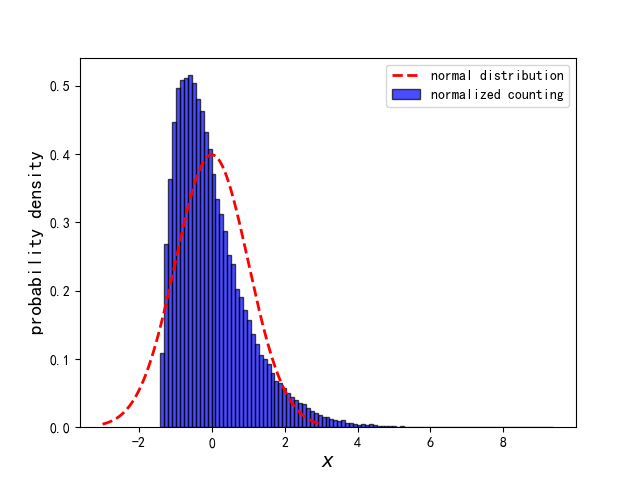
\includegraphics[width=0.45\textwidth]{../result/exp_2.png}}
					\subfigure[N=5]{
						
						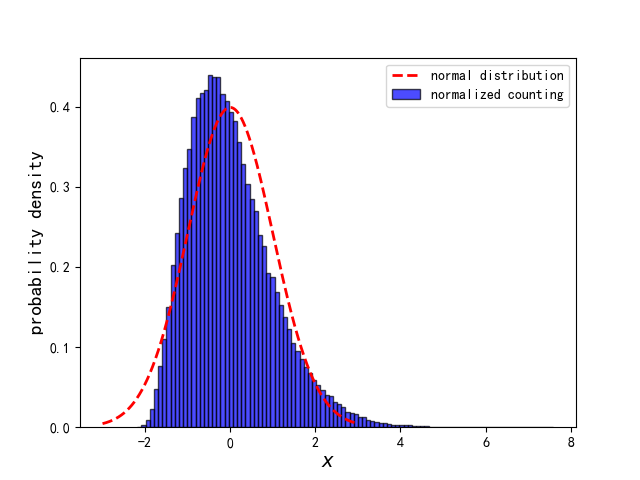
\includegraphics[width=0.45\textwidth]{../result/exp_5.png}}
						\subfigure[N=10]{
						
						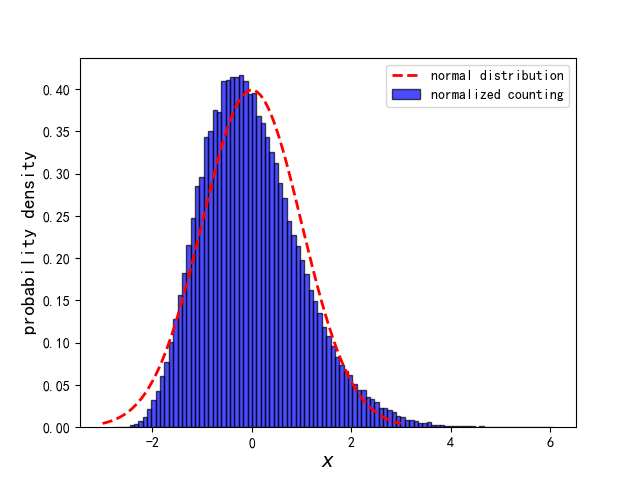
\includegraphics[width=0.45\textwidth]{../result/exp_10.png}}
							\subfigure[N=100]{
							
							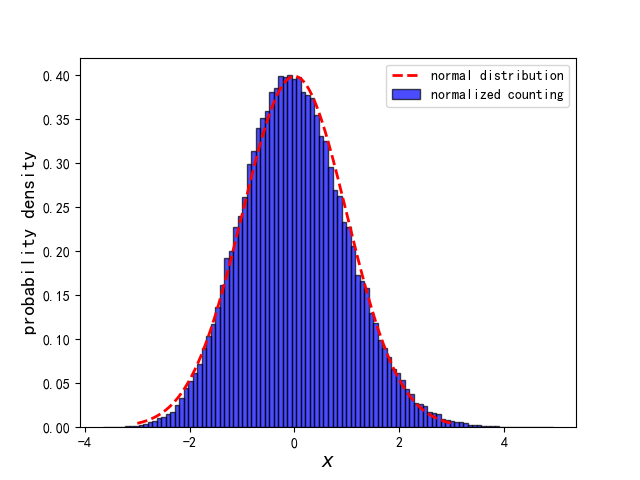
\includegraphics[width=0.45\textwidth]{../result/exp_100.png}}
						\subfigure[N=1000]{
						
						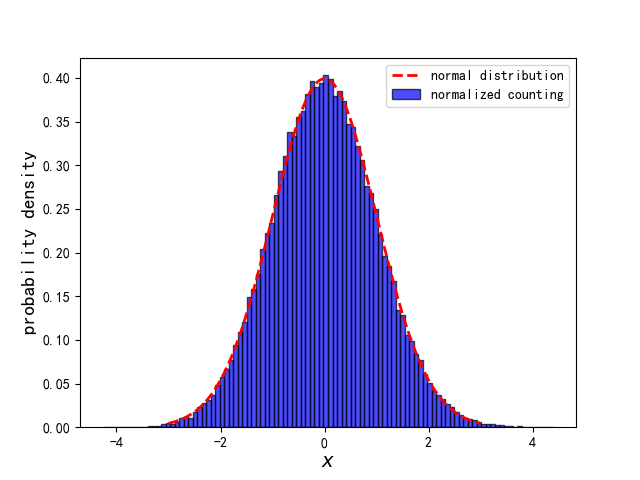
\includegraphics[width=0.45\textwidth]{../result/exp_1000.png}}	
					\caption{不同$N$下面的$Y$分布情况}
					\label{Fig.main}
				\end{figure}
			
	可见,当$N=100$时已经和正态分布曲线非常吻合了。
	\newpage
	\subsection{Poisson分布}
	$$p(x=k)=\frac{1}{k!}e^{-1}$$
	\begin{figure}[H]
		\centering  %图片全局居中
		\subfigure[N=2]{
			
			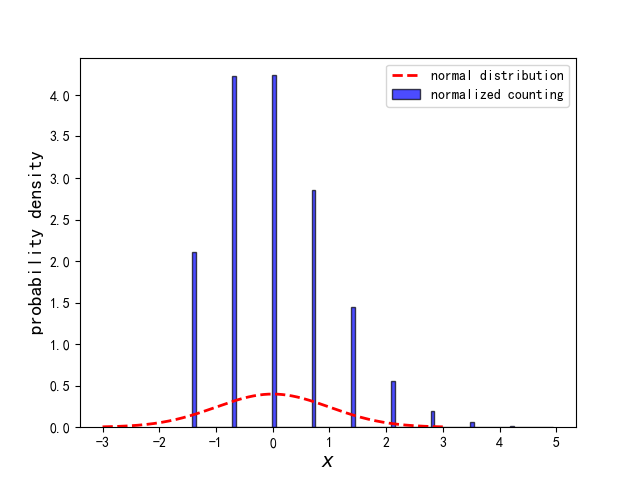
\includegraphics[width=0.45\textwidth]{../result/poi_2.png}}
		\subfigure[N=5]{
			
			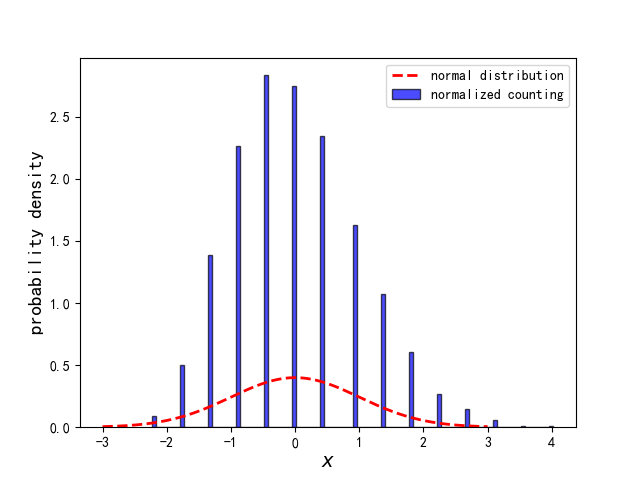
\includegraphics[width=0.45\textwidth]{../result/poi_5.png}}
		\subfigure[N=10]{
			
			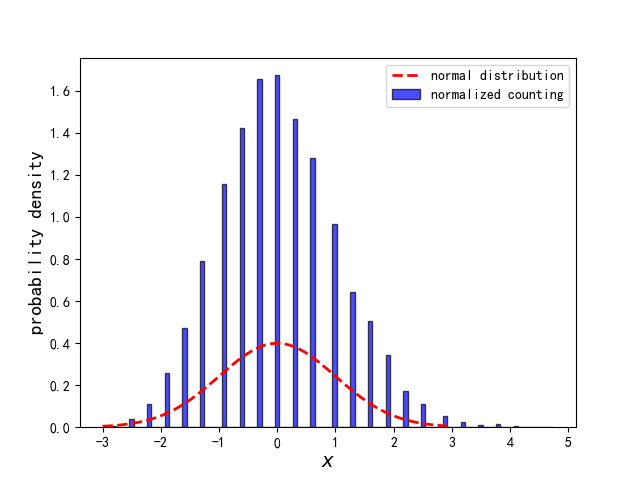
\includegraphics[width=0.45\textwidth]{../result/poi_10.png}}
		\subfigure[N=1000]{
			
			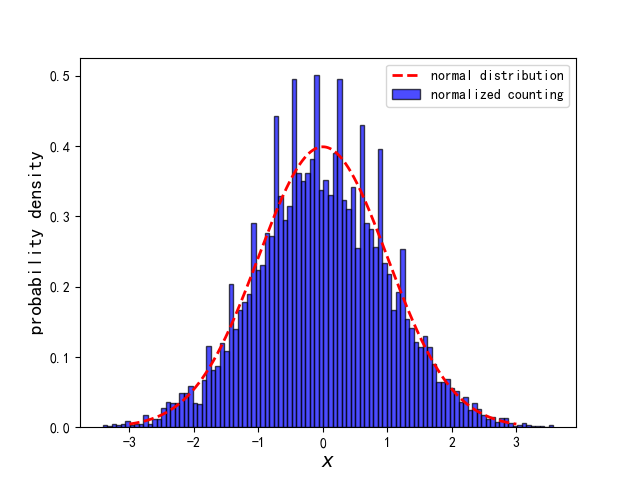
\includegraphics[width=0.45\textwidth]{../result/poi_1000.png}}
		\subfigure[N=10000]{
			
			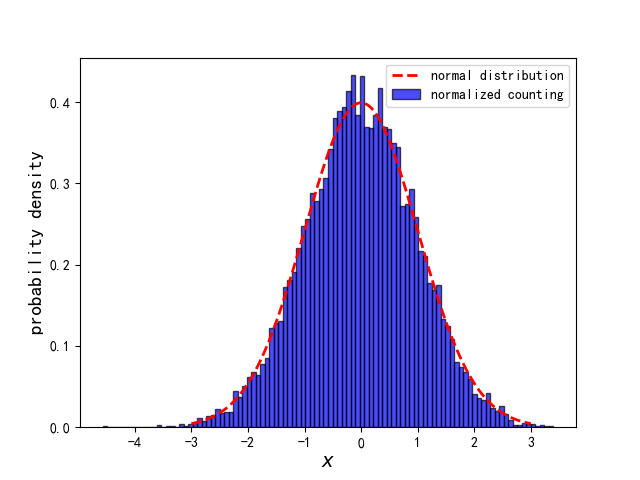
\includegraphics[width=0.45\textwidth]{../result/poi_10000.png}}	
		\caption{不同$N$下面的$Y$分布情况}
	\end{figure}

	\begin{flushleft}
		\quad 对于离散型的$poisson$分布,可见$Y$收敛到正态分布的速度要比连续性的指数分布慢得多,直到$N=10000$时在中心处仍有少许“毛刺”。
	\end{flushleft}

\subsection{自设分布}
$$p(x)=1.81915\frac{e^{-x}}{{(x-2)^2}}\quad (-1\leq x\leq1)$$
\begin{figure}[H]
	\centering  %图片全局居中
	\subfigure[N=2]{
		
		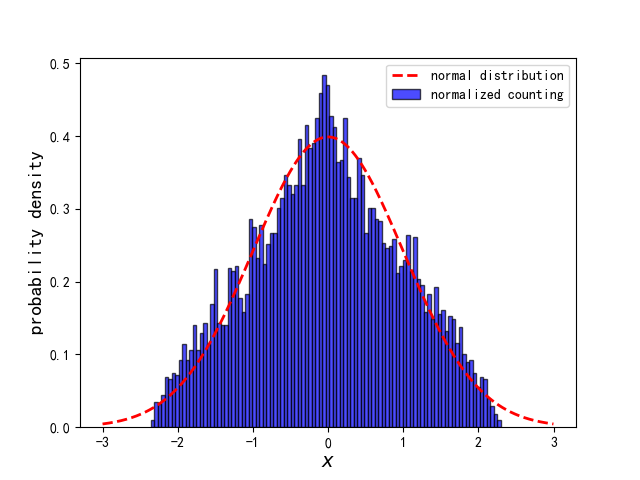
\includegraphics[width=0.45\textwidth]{../result/self_2.png}}
	\subfigure[N=5]{
		
		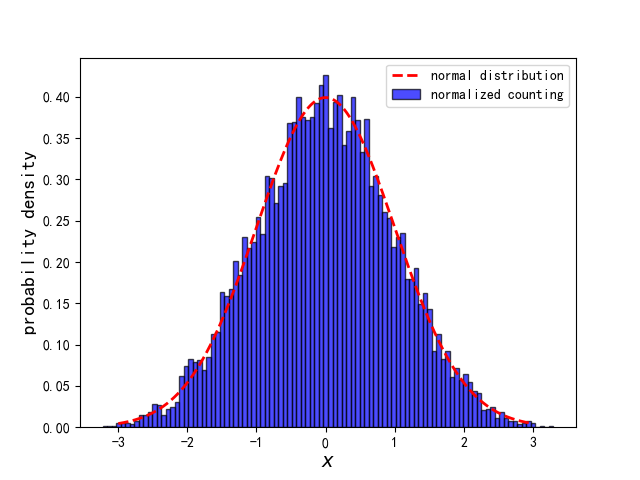
\includegraphics[width=0.45\textwidth]{../result/self_5.png}}
	
	\subfigure[N=10]{
		
		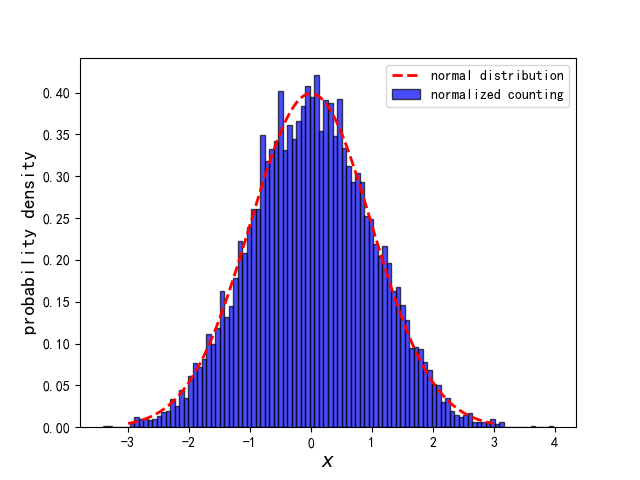
\includegraphics[width=0.45\textwidth]{../result/self_10.png}}
	\subfigure[N=1000]{
		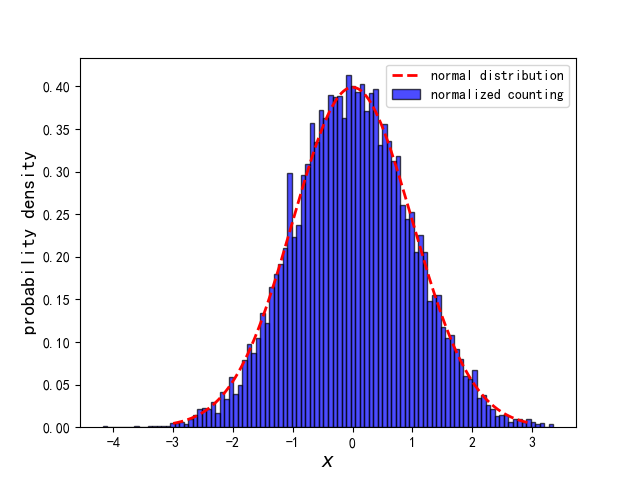
\includegraphics[width=0.45\textwidth]{../result/self_1000.png}}
		
	\caption{不同$N$下面的$Y$分布情况}
\end{figure}

\begin{flushleft}
	\quad 对于这个自设分布,当$N=1000$时有比较好的拟合效果,但是相比指数分布的还是收敛略慢。不过相比之下,当$N=5$时也已经比较靠近正态分布函数了,其原因可能是本来的分布函数在$(-1,1)$上的对称性比指数分布的要高。
\end{flushleft}
%		\begin{figure}[H]
%		\centering  %图片全局居中
%		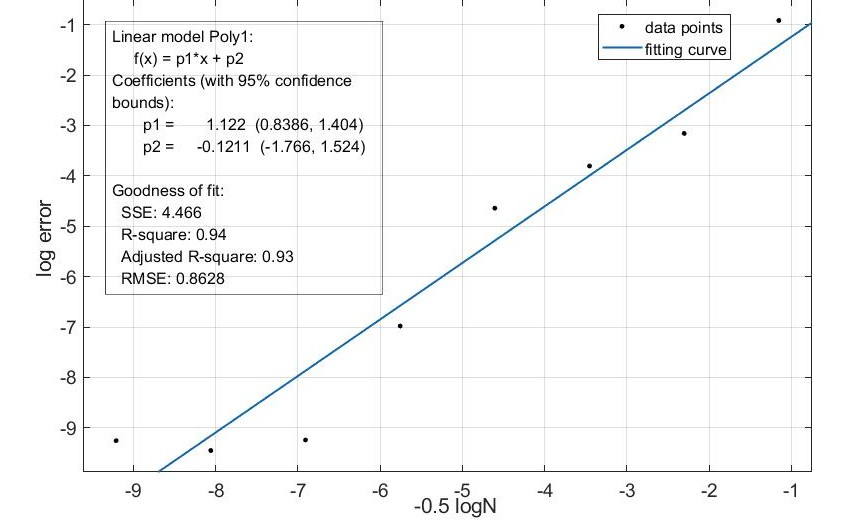
\includegraphics[width=6in]{../figure/single.jpg}
%		\caption{$log(\epsilon)-log(\frac{1}{\sqrt{N}})$}
%	\end{figure}
	

%	\begin{figure}[H]
%		\centering  %图片全局居中
%		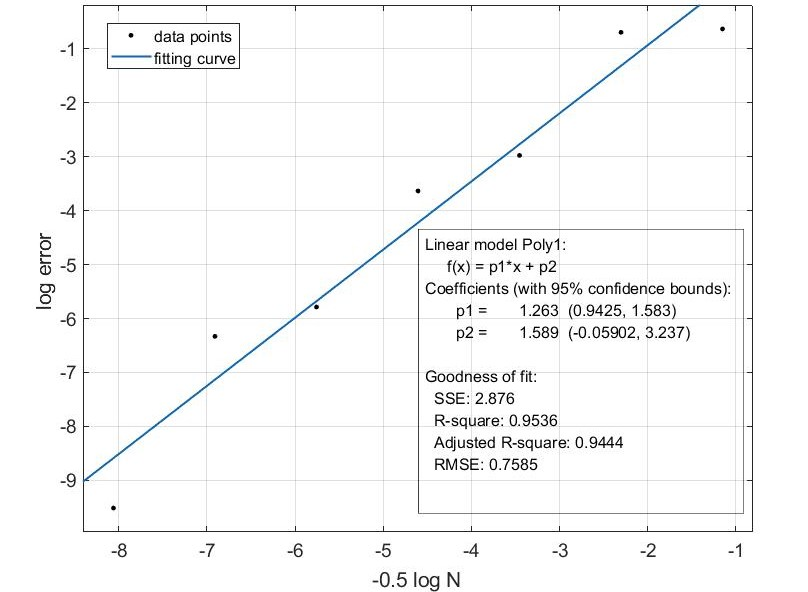
\includegraphics[width=6in]{../figure/multi.jpg}
%		\caption{$log(\epsilon)-log(\frac{1}{\sqrt{N}})$}
%	\end{figure}

	\newpage
	\section{总结}
	\begin{itemize}
		\item 本次实验通过不同分布下的随机序列验证了中心极限定理成立。
		\item 中心极限定理给出了计算物理中估计误差非常重要的一个公式:
		$$\langle x \rangle \sim N\left(\mu,\frac{\sigma_x}{\sqrt{N}}\right)$$
		这表示当$N$足够大时,误差$\sigma\sim\sigma_x/\sqrt{N}$
	\end{itemize}
	\clearpage
\end{document}